\documentclass[a4paper, amsfonts, amssymb, amsmath, reprint, showkeys, nofootinbib, twoside]{revtex4-1}
\usepackage[english]{babel}
\usepackage[utf8]{inputenc}
\usepackage[colorinlistoftodos, color=green!40, prependcaption]{todonotes}
%\input{preamble}
\usepackage[pdftex, pdftitle={Article}, pdfauthor={Author}]{hyperref} % For hyperlinks in the PDF
\usepackage{siunitx}
\usepackage{braket}
\usepackage{xfrac}
\usepackage{caption}
\usepackage{subcaption}
\captionsetup{justification=raggedright,singlelinecheck=false}
\newcommand\editremark[1]{{\color{red}#1}}
%\setlength{\marginparwidth}{2.5cm}
%\usepackage{biblatex}
%\addbibresource{Reference.bib}
\bibliographystyle{apsrev4-1}
\begin{document}
\title{Numerical modeling of spiral resonators}

\author{Elizabeth Champion}
\affiliation{Department of Physics and Astronomy, University of Rochester}

\date{\today} % Leave empty to omit a date

\maketitle

\section{Spiral geometry}

A spiral is specified by three parameters: its external radius $R_e$, internal radius $R_i$, and pitch $p$.
The shape of the spiral is given in polar coordinates by
\begin{equation} \label{eq:arch}
    \rho(\phi) = R_e (1 - \alpha \phi)
\end{equation}
where
\[
    \alpha = \frac {p} {2 \pi R_e}.
\]
Then the maximum value of $\phi$ is given by setting $\rho = R_i$:
\[
    \phi_{\rm max} = \frac {1} {\alpha} \left ( 1 - \frac {R_i} {R_e} \right ).
\]

We specify position along the length of the spiral in terms of a coordinate $s$, which has its origin at the outside of the spiral.
It will be useful later to be able to express the angular position $\phi$ as a function of $s$, which we will do now.
Consider a differential element of length along the spiral $ds$, of radial distance from the center of the spiral $d\rho$, and of angle $d\phi$.
These are related by
\[
    ds^2 = d\rho^2 + \rho^2 d\phi^2,
\]
or using Eq (\ref{eq:arch}) to express $d\rho$ in terms of $d\phi$, 
\begin{equation} \label{eq:diffeq}
    \left ( \frac {ds} {d\phi} \right )^2 = \alpha^2 R_e^2 + \rho^2.
\end{equation}
It is not straightforward to solve this exactly, and numerical integration would add computational cost to the model; however, we can approximate the solution using a geometric argument.
Consider the area occupied by a length $s$ of a given spiral.
This can be approximated as the area between concentric circles,
\[
    {\rm Area} = \pi (R_e^2 - \rho(s)^2),
\]
but we can also approximate it as the length of the spiral multiplied by the width of each turn,
\[
    {\rm Area} = p s;
\]
setting these two equal to each other yields an approximation for $\phi(s)$:
\[
    \phi(s) = \frac {1} {\alpha} \left [ 1 - \sqrt{1 - \frac {2 \alpha s} {R_e}} \right ].
\]
We can check that this approximation is valid by computing $ds/d\phi$ and comparing it to Eq. (\ref{eq:diffeq}).
Doing so we find
\[
    \frac {ds} {d\phi} = \rho^2;
\]
the approximation is therefore valid when the difference between these is negligible, i.e.
\[
    \rho \gg \alpha R_e = \frac {p} {2\pi};
\]
that is, the radial distance we are considering must be larger than the pitch, which is generally satisfied for the spirals we consider.
Figure \ref{fig:phi} shows a representative example which demonstrates the very good agreement between this approximation and the result of a numerical integration.

\begin{figure}
    \centering
    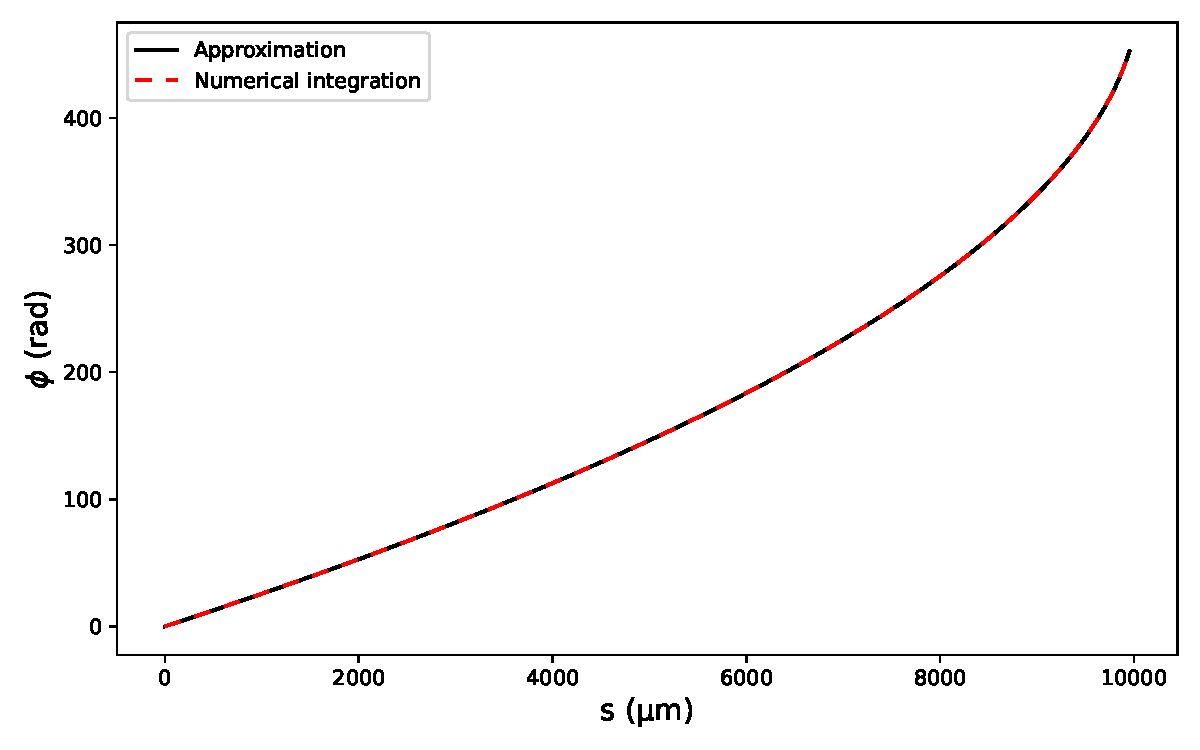
\includegraphics[width=\columnwidth]{phi.pdf}
    \caption{Comparison between approximate $\phi(s)$ and the value computed using numerical integration.}
    \label{fig:phi}
\end{figure}

\section{Resonant frequency calculation}

Following \cite{maleeva_electrodynamics_2014, maleeva_electrodynamics_2015}, we express the vector potential due to the spiral at a point $(r, \theta)$ in the plane of the spiral as
\begin{equation} \label{eq:vec}
    \vec{A}(r, \theta) = \frac {\mu_0 I} {4 \pi} \int \frac {e^{-i k R}} {R} \psi(s) d\vec{s}
\end{equation}
where $k = \omega / c_eff$, $\psi(s)$ is the current distribution along the spiral, and $I$ is the amplitude of the current.
The distance $R$ is given by
\[
    R = \sqrt{r^2 + R_e^2 (1 - \alpha \phi)^2 - 2 r R_e (1 - \alpha \phi) \cos(\phi - \theta)};
\]
note that the $\phi$ in this equation is the angle corresponding to position $s$ along the spiral, hence the need for our approximation.

The electric field components in the plane of the spiral are
\[
    E_r = \frac {1} {i \omega \epsilon_0 \mu_0} \frac {d} {dr} \left [ \frac {1} {r} \frac {d} {dr} (r A_r)  \right ]
\]
and
\[
    E_\theta = -i \omega A_\theta;
\]
the boundary condition that must be satisfied is for the electric field along the direction of the spiral to be zero,
\begin{equation}\label{eq:bc1}
    R_e \alpha E_r + r E_\theta = 0,
\end{equation}
and it must also be the case that the current at both ends of the spiral is zero, i.e.
\begin{equation} \label{eq:bc2}
    \psi(0) = \psi(s_{\rm max}) = 0.
\end{equation}

In the cases where $R_e - R_i \ll R_e$ \cite{maleeva_electrodynamics_2014} or $R_i = 0$ \cite{maleeva_electrodynamics_2015}, Maleeva et al. apply a set of approximations that allow for an analytic solution for the frequency $\omega$ as well as $\psi(s)$.
In our case, however, we wish to model the intermediate region, where these approximations are no longer valid.
We therefore make no approximations and instead solve for $\omega$ and $\psi(s)$ numerically.
The current distribution $\psi(s)$ is parameterized as a sum of sine functions:
\[
    \psi(s) = \sum_n c_n \sin \left ( \frac {n \pi s} {s_{\rm max}} \right )
\]
up to some finite order; note that this parameterization automatically enforces boundary condition (\ref{eq:bc2}).
The process for finding a numerical solution is:
\begin{enumerate}
    \item Given values for $\omega$ and each coefficient $c_n$, compute the vector potential and the electric field due to the spiral via numerical integration of Eq. (\ref{eq:vec}) and numerical differentiation of the result, respectively.
        This is done for a set of points drawn from the area of the spiral, $\{(r_i, \theta_i)\}$.
    \item At each of these points compute $E_i^{||} = R_e \alpha E_{r_i} + r_i E_{\theta_i}$, i.e. the electric field in the direction along the wire
\end{enumerate}

\bibliography{citations}

\end{document}
